\section{Descrizione dei Dati} % matrici
Di seguito verranno trattate le diverse matrici utilizzate durante la sperimentazione. In particolar modo si vuole sottolineare che esse fanno parte della \href{
https://sparse.tamu.edu/}{SuiteSparse Matrix Collection} che colleziona matrici sparse derivanti da
applicazioni di problemi reali come: ingegneria strutturale, fluidodinamica, elettromagnetismo,
termodinamica, computer graphics/vision, network e grafi. \footnote{Nei dati riportati ricorrerà spesso la sigla CFDP, acronimo di "Computational Fluid Dynamics Problem".}
%######################################################################%
%||                                                                  %||
%||                                                                  %||
%||                            NEW MATRIX                            %||
%||                                                                  %||
%||                                                                  %||
%######################################################################%

\subsection{Flan-1565}
\begin{table}[h!]
	\begin{minipage}{0.5\linewidth}
		\caption{Flan-1565 Information}
		\label{table:Flan-1565}
		\centering
        \begin{tabular}{ll}
\midrule
                       Name &              Flan\_1565 \\
                      Group &                  Janna \\
                  Matrix ID &                   2544 \\
                   Num Rows &                1564794 \\
                   Num Cols &                1564794 \\
                   Nonzeros &              114165372 \\
            Pattern Entries &              117406044 \\
                       Kind &     Structural Problem \\
                  Symmetric &                    Yes \\
                       Date &                   2011 \\
                     Author & C. Janna, M. Ferronato \\
                     Editor &               T. Davis \\
            Structural Rank &                1564794 \\
       Structural Rank Full &                   true \\
          Num Dmperm Blocks &                      1 \\
Strongly Connect Components &                      1 \\
         Num Explicit Zeros &                3240672 \\
           Pattern Symmetry &                   100\% \\
           Numeric Symmetry &                   100\% \\
         Cholesky Candidate &                    yes \\
          Positive Definite &                    yes \\
                       Type &                   real \\
\bottomrule
\end{tabular}

	\end{minipage}\hfill
	\begin{minipage}{0.45\linewidth}
		\centering
		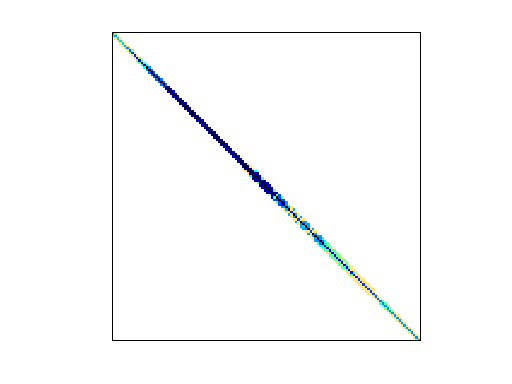
\includegraphics[width=1\textwidth]{figs/Flan_1565.png}
		\captionof{figure}{Flan-1565}
		\label{fig:Flan-1565}
	\end{minipage}
\end{table}

%######################################################################%
%||                                                                  %||
%||                                                                  %||
%||                            NEW MATRIX                            %||
%||                                                                  %||
%||                                                                  %||
%######################################################################%

\subsection{StocF-1465}
\begin{table}[ht!]
	\begin{minipage}{0.5\linewidth}
		\caption{StocF-1465 Information}
		\label{table:StocF-1465}
		\centering
        \begin{tabular}{ll}
\midrule
                       Name &                           StocF-1465 \\
                      Group &                                Janna \\
                  Matrix ID &                                 2547 \\
                   Num Rows &                              1465137 \\
                   Num Cols &                              1465137 \\
                   Nonzeros &                             21005389 \\
            Pattern Entries &                             21005389 \\
                       Kind & CFDP \\
                  Symmetric &                                  Yes \\
                       Date &                                 2011 \\
                     Author &               C. Janna, M. Ferronato \\
                     Editor &                             T. Davis \\
            Structural Rank &                              1465137 \\
       Structural Rank Full &                                 true \\
          Num Dmperm Blocks &                                29105 \\
Strongly Connect Components &                                29105 \\
         Num Explicit Zeros &                                    0 \\
           Pattern Symmetry &                                 100\% \\
           Numeric Symmetry &                                 100\% \\
         Cholesky Candidate &                                  yes \\
          Positive Definite &                                  yes \\
                       Type &                                 real \\
\bottomrule
\end{tabular}

	\end{minipage}\hfill
	\begin{minipage}{0.45\linewidth}
		\centering
		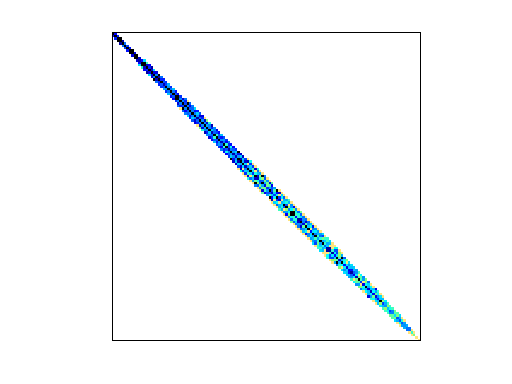
\includegraphics[width=1\textwidth]{figs/StocF-1465.png}
		\captionof{figure}{StocF-1465}
		\label{fig:StocF-1465}
	\end{minipage}
\end{table}


%######################################################################%
%||                                                                  %||
%||                                                                  %||
%||                            NEW MATRIX                            %||
%||                                                                  %||
%||                                                                  %||
%######################################################################%

\subsection{cfd2}
\begin{table}[h!]
	\begin{minipage}{0.5\linewidth}
		\caption{cfd2 Information}
		\label{table:cfd2}
		\centering
        \begin{tabular}{ll}
\midrule
                       Name &                                 cfd2 \\
                      Group &                             Rothberg \\
                  Matrix ID &                                  805 \\
                   Num Rows &                               123440 \\
                   Num Cols &                               123440 \\
                   Nonzeros &                              3085406 \\
            Pattern Entries &                              3087898 \\
                       Kind & CFDP \\
                  Symmetric &                                  Yes \\
                       Date &                                 1997 \\
                     Author &                          E. Rothberg \\
                     Editor &                             T. Davis \\
            Structural Rank &                               123440 \\
       Structural Rank Full &                                 true \\
          Num Dmperm Blocks &                                    1 \\
Strongly Connect Components &                                    1 \\
         Num Explicit Zeros &                                 2492 \\
           Pattern Symmetry &                                 100\% \\
           Numeric Symmetry &                                 100\% \\
         Cholesky Candidate &                                  yes \\
          Positive Definite &                                  yes \\
                       Type &                                 real \\
\bottomrule
\end{tabular}

	\end{minipage}\hfill
	\begin{minipage}{0.45\linewidth}
		\centering
		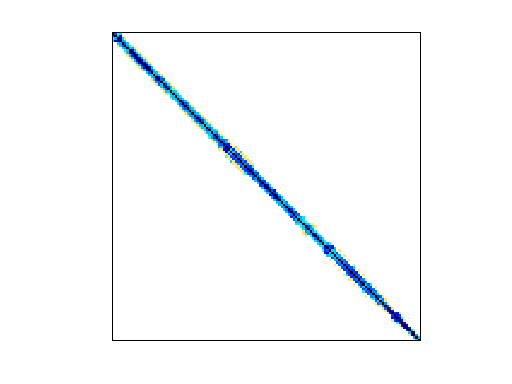
\includegraphics[width=1\textwidth]{figs/cfd2.png}
		\captionof{figure}{cfd2}
		\label{fig:cfd2}
	\end{minipage}
\end{table}


%######################################################################%
%||                                                                  %||
%||                                                                  %||
%||                            NEW MATRIX                            %||
%||                                                                  %||
%||                                                                  %||
%######################################################################%
\subsection{cfd1}
\begin{table}[h!]
	\begin{minipage}{0.5\linewidth}
		\caption{cdf1 Information}
		\label{table:cdf1}
		\centering
        \begin{tabular}{ll}
\midrule
                       Name &                                 cfd1 \\
                      Group &                             Rothberg \\
                  Matrix ID &                                  804 \\
                   Num Rows &                                70656 \\
                   Num Cols &                                70656 \\
                   Nonzeros &                              1825580 \\
            Pattern Entries &                              1828364 \\
                       Kind & CFDP \\
                  Symmetric &                                  Yes \\
                       Date &                                 1997 \\
                     Author &                          E. Rothberg \\
                     Editor &                             T. Davis \\
            Structural Rank &                                70656 \\
       Structural Rank Full &                                 true \\
          Num Dmperm Blocks &                                    1 \\
Strongly Connect Components &                                    1 \\
         Num Explicit Zeros &                                 2784 \\
           Pattern Symmetry &                                 100\% \\
           Numeric Symmetry &                                 100\% \\
         Cholesky Candidate &                                  yes \\
          Positive Definite &                                  yes \\
                       Type &                                 real \\
\bottomrule
\end{tabular}

	\end{minipage}\hfill
	\begin{minipage}{0.45\linewidth}
		\centering
		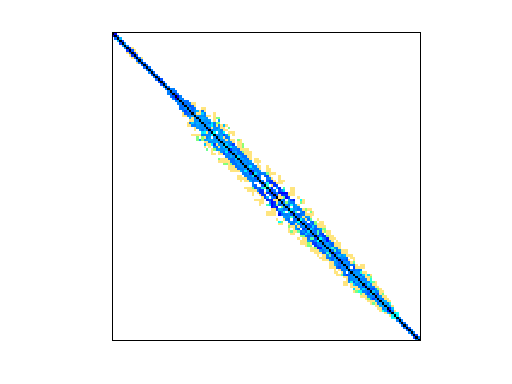
\includegraphics[width=1\textwidth]{figs/cfd1.png}
		\captionof{figure}{cdf1}
		\label{fig:cdf1}
	\end{minipage}
\end{table}



%######################################################################%
%||                                                                  %||
%||                                                                  %||
%||                            NEW MATRIX                            %||
%||                                                                  %||
%||                                                                  %||
%######################################################################%
\subsection{G3-circuit}
\begin{table}[h!]
	\begin{minipage}{0.5\linewidth}
		\caption{G3-circuit Information}
		\label{table:cdf1}
		\centering
        \begin{tabular}{ll}
\midrule
                       Name &                 G3\_circuit \\
                      Group &                        AMD \\
                  Matrix ID &                       1421 \\
                   Num Rows &                    1585478 \\
                   Num Cols &                    1585478 \\
                   Nonzeros &                    7660826 \\
            Pattern Entries &                    7660826 \\
                       Kind & Circuit Simulation Problem \\
                  Symmetric &                        Yes \\
                       Date &                       2006 \\
                     Author &                 U. Okuyucu \\
                     Editor &                   T. Davis \\
            Structural Rank &                    1585478 \\
       Structural Rank Full &                       true \\
          Num Dmperm Blocks &                          1 \\
Strongly Connect Components &                          1 \\
         Num Explicit Zeros &                          0 \\
           Pattern Symmetry &                       100\% \\
           Numeric Symmetry &                       100\% \\
         Cholesky Candidate &                        yes \\
          Positive Definite &                        yes \\
                       Type &                       real \\
\bottomrule
\end{tabular}

	\end{minipage}\hfill
	\begin{minipage}{0.45\linewidth}
		\centering
		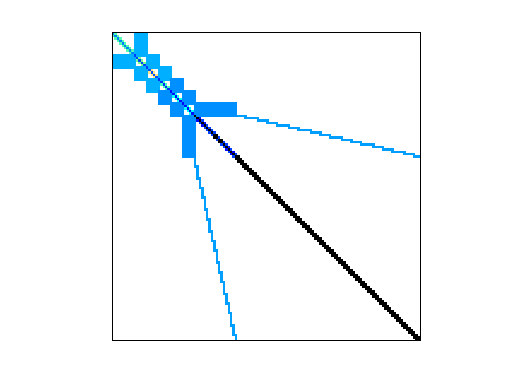
\includegraphics[width=1\textwidth]{figs/G3_circuit.png}
		\captionof{figure}{G3-circuit}
		\label{fig:G3-circuit}
	\end{minipage}
\end{table}



%######################################################################%
%||                                                                  %||
%||                                                                  %||
%||                            NEW MATRIX                            %||
%||                                                                  %||
%||                                                                  %||
%######################################################################%
\subsection{Parabolic Fem}
\begin{table}[h!]
	\begin{minipage}{0.5\linewidth}
		\caption{Parabolic Fem Information}
		\label{table:Parabolic Fem}
		\centering
        \begin{tabular}{ll}
\midrule
                       Name &                        parabolic\_fem \\
                      Group &                             Wissgott \\
                  Matrix ID &                                 1853 \\
                   Num Rows &                               525825 \\
                   Num Cols &                               525825 \\
                   Nonzeros &                              3674625 \\
            Pattern Entries &                              3674625 \\
                       Kind & CFDP \\
                  Symmetric &                                  Yes \\
                       Date &                                 2007 \\
                     Author &                          P. Wissgott \\
                     Editor &                             T. Davis \\
            Structural Rank &                               525825 \\
       Structural Rank Full &                                 true \\
          Num Dmperm Blocks &                                    1 \\
Strongly Connect Components &                                    1 \\
         Num Explicit Zeros &                                    0 \\
           Pattern Symmetry &                                 100\% \\
           Numeric Symmetry &                                 100\% \\
         Cholesky Candidate &                                  yes \\
          Positive Definite &                                  yes \\
                       Type &                                 real \\
\bottomrule
\end{tabular}

	\end{minipage}\hfill
	\begin{minipage}{0.45\linewidth}
		\centering
		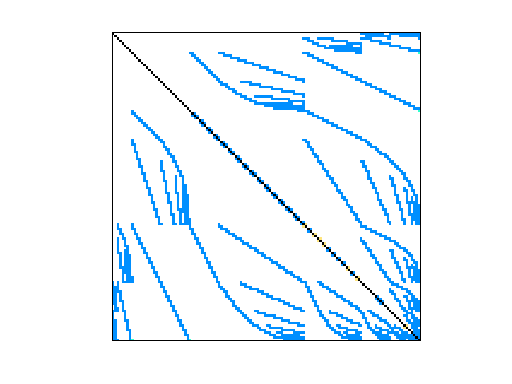
\includegraphics[width=1\textwidth]{figs/parabolic_fem.png}
		\captionof{figure}{Parabolic Fem}
		\label{fig:Parabolic Fem}
	\end{minipage}
\end{table}



%######################################################################%
%||                                                                  %||
%||                                                                  %||
%||                            NEW MATRIX                            %||
%||                                                                  %||
%||                                                                  %||
%######################################################################%
\subsection{apache2}
\begin{table}[h!]
	\begin{minipage}{0.5\linewidth}
		\caption{apache2 Information}
		\label{table:apache2}
		\centering
        \begin{tabular}{ll}
\midrule
                       Name &                   apache2 \\
                      Group &                 GHS\_psdef \\
                  Matrix ID &                      1423 \\
                   Num Rows &                    715176 \\
                   Num Cols &                    715176 \\
                   Nonzeros &                   4817870 \\
            Pattern Entries &                   4817870 \\
                       Kind &        Structural Problem \\
                  Symmetric &                       Yes \\
                       Date &                      2006 \\
                     Author &                       NaN \\
                     Editor & N. Gould, Y. Hu, J. Scott \\
            Structural Rank &                    715176 \\
       Structural Rank Full &                      true \\
          Num Dmperm Blocks &                         1 \\
Strongly Connect Components &                         1 \\
         Num Explicit Zeros &                         0 \\
           Pattern Symmetry &                      100\% \\
           Numeric Symmetry &                      100\% \\
         Cholesky Candidate &                       yes \\
          Positive Definite &                       yes \\
                       Type &                      real \\
\bottomrule
\end{tabular}

	\end{minipage}\hfill
	\begin{minipage}{0.45\linewidth}
		\centering
		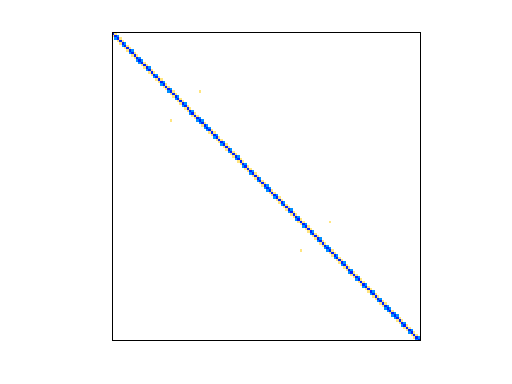
\includegraphics[width=1\textwidth]{figs/apache2.png}
		\captionof{figure}{apache2}
		\label{fig:apache2}
	\end{minipage}
\end{table}



%######################################################################%
%||                                                                  %||
%||                                                                  %||
%||                            NEW MATRIX                            %||
%||                                                                  %||
%||                                                                  %||
%######################################################################%
\subsection{shallow water1}
\begin{table}[h!]
	\begin{minipage}{0.5\linewidth}
		\caption{shallow water1 Information}
		\label{table:shallow water1}
		\centering
        \begin{tabular}{ll}
\midrule
                       Name &                       shallow\_water1 \\
                      Group &                            MaxPlanck \\
                  Matrix ID &                                 2261 \\
                   Num Rows &                                81920 \\
                   Num Cols &                                81920 \\
                   Nonzeros &                               327680 \\
            Pattern Entries &                               327680 \\
                       Kind & CFDP \\
                  Symmetric &                                  Yes \\
                       Date &                                 2009 \\
                     Author &               K. Leppkes, U. Naumann \\
                     Editor &                             T. Davis \\
            Structural Rank &                                81920 \\
       Structural Rank Full &                                 true \\
          Num Dmperm Blocks &                                    1 \\
Strongly Connect Components &                                    1 \\
         Num Explicit Zeros &                                    0 \\
           Pattern Symmetry &                                 100\% \\
           Numeric Symmetry &                                 100\% \\
         Cholesky Candidate &                                  yes \\
          Positive Definite &                                  yes \\
                       Type &                                 real \\
\bottomrule
\end{tabular}

	\end{minipage}\hfill
	\begin{minipage}{0.45\linewidth}
		\centering
		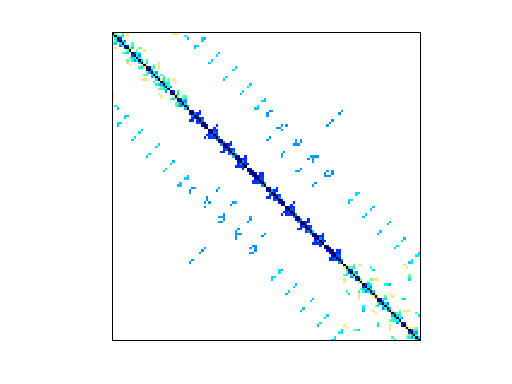
\includegraphics[width=1\textwidth]{figs/shallow_water1.png}
		\captionof{figure}{shallow water1}
		\label{fig:shallow water1}
	\end{minipage}
\end{table}




%######################################################################%
%||                                                                  %||
%||                                                                  %||
%||                            NEW MATRIX                            %||
%||                                                                  %||
%||                                                                  %||
%######################################################################%
\subsection{ex15}
\begin{table}[h!]
	\begin{minipage}{0.5\linewidth}
		\caption{ex15 Information}
		\label{table:ex15}
		\centering
        \begin{tabular}{ll}
\midrule
                       Name &                                 ex15 \\
                      Group &                                FIDAP \\
                  Matrix ID &                                  413 \\
                   Num Rows &                                 6867 \\
                   Num Cols &                                 6867 \\
                   Nonzeros &                                98671 \\
            Pattern Entries &                                98671 \\
                       Kind & CFDP \\
                  Symmetric &                                  Yes \\
                       Date &                                 1994 \\
                     Author &                   A. Baggag, Y. Saad \\
                     Editor &                   A. Baggag, Y. Saad \\
            Structural Rank &                                 6867 \\
       Structural Rank Full &                                 true \\
          Num Dmperm Blocks &                                    2 \\
Strongly Connect Components &                                    2 \\
         Num Explicit Zeros &                                    0 \\
           Pattern Symmetry &                                 100\% \\
           Numeric Symmetry &                                 100\% \\
         Cholesky Candidate &                                  yes \\
          Positive Definite &                                  yes \\
                       Type &                                 real \\
\bottomrule
\end{tabular}

	\end{minipage}\hfill
	\begin{minipage}{0.45\linewidth}
		\centering
		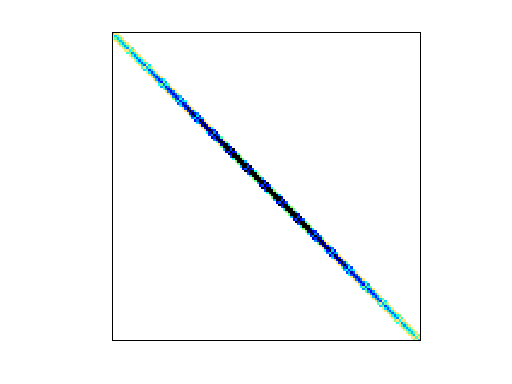
\includegraphics[width=1\textwidth]{figs/ex15.png}
		\captionof{figure}{ex15}
		\label{fig:ex15}
	\end{minipage}
\end{table}
